% !TeX encoding = UTF-8
% !TeX program = XeLaTeX
% !TeX spellcheck = LaTeX

\documentclass[a4paper]{article}

\usepackage{amsmath,amsfonts,amssymb}
\usepackage{mathrsfs}
\usepackage{bm}
\usepackage{extarrows}
\usepackage{geometry}
\usepackage{ntheorem}
\usepackage{hyperref}
\usepackage[ruled]{algorithm2e}
\usepackage{caption,subcaption}
\usepackage{tikz}

\usetikzlibrary{automata}

\geometry{left=2cm,right=2cm,top=2cm,bottom=2cm}

\def\UrlBreaks{\do\A\do\B\do\C\do\D\do\E\do\F\do\G\do\H\do\I\do\J\do\K\do\L\do\M\do\N\do\O\do\P\do\Q\do\R\do\S\do\T\do\U\do\V\do\W\do\X\do\Y\do\Z\do\[\do\\\do\]\do\^\do\_\do\`\do\a\do\b\do\c\do\d\do\e\do\f\do\g\do\h\do\i\do\j\do\k\do\l\do\m\do\n\do\o\do\p\do\q\do\r\do\s\do\t\do\u\do\v\do\w\do\x\do\y\do\z\do\0\do\1\do\2\do\3\do\4\do\5\do\6\do\7\do\8\do\9\do\.\do\@\do\\\do\/\do\!\do\_\do\|\do\;\do\>\do\]\do\)\do\,\do\?\do\'\do+\do\=\do\#}

\newtheorem{theorem}{Theorem}
\newtheorem{lemma}{Lemma}
\newtheorem{proposition}{Proposition}
\newtheorem{corollary}{Corollary}
\newtheorem{claim}{Claim}
\newtheorem{conjecture}{conjecture}
\newtheorem{definition}{Definition}
\newtheorem{construction}{Construction}
\newtheorem*{proof}{Proof}
\newtheorem*{answer}{Answer}
\newtheorem*{example}{Example}
\newtheorem*{counterexample}{Counterexample}

\newenvironment{exercise}[1]{
	\par
	\noindent\textbf{Exercise #1.}\quad
}{
	\par
	\bigskip
}
\newenvironment{problem}[1]{
	\par
	\noindent\textbf{Problem #1.}\quad
}{
	\par
	\bigskip
}

\DeclareMathAccent{\widehat}{\mathord}{largesymbols}{"62}
\DeclareMathOperator*{\argmax}{\arg\,\max}
\DeclareMathOperator*{\argmin}{\arg\,\min}
\DeclareMathOperator{\E}{\mathbb E}
\DeclareMathOperator{\Var}{\mathrm{Var}}
\DeclareMathOperator{\tr}{\mathrm{tr}}
\DeclareMathOperator{\poly}{\mathrm{poly}}
\newcommand{\abs}[1]{\left| #1 \right|}
\newcommand{\vabs}[1]{\left\| #1 \right\|}
\newcommand{\abra}[1]{\left\langle #1 \right\rangle}
\newcommand{\pbra}[1]{\left( #1 \right)}
\newcommand{\cbra}[1]{\left\{ #1 \right\}}
\newcommand{\sbra}[1]{\left[ #1 \right]}
\newcommand{\floorbra}[1]{\left\lfloor #1 \right\rfloor}
\newcommand{\ceilbra}[1]{\left\lceil #1 \right\rceil}
\newcommand{\bin}{\{0,1\}}
\newcommand{\ZPP}{\mathtt{ZPP}}
\newcommand{\RP}{\mathtt{RP}}
\newcommand{\coRP}{\mathtt{co}\text{-}\mathtt{RP}}
\newcommand{\per}{\text{per}}
\newcommand{\sgn}{\text{sgn}}
\newcommand{\Fbb}{\mathbb{F}}
\newcommand{\Nbb}{\mathbb{N}}
\newcommand{\Rbb}{\mathbb{R}}
\newcommand{\Zbb}{\mathbb{Z}}
\newcommand{\Sset}{\mathbb{S}}
\newcommand{\Acal}{\mathcal{A}}
\newcommand{\Bcal}{\mathcal{B}}
\newcommand{\Ccal}{\mathcal{C}}
\newcommand{\Fcal}{\mathcal{F}}
\newcommand{\Gcal}{\mathcal{G}}
\newcommand{\qd}[2]{{\left(\frac{#1}{#2}\right)}}

\bibliographystyle{plainnat}

\title{Exercise Set --- Chapter $2$}
\date{}

\begin{document}

\maketitle

\begin{exercise}{2.2.5}\hspace{0pt}\\
\textbf{a)} I think string of length less than $5$ is also acceptable. And I believe the question means every $5$ consecutive characters should contain at least two $0$'s. For example, string $001111$ 
is not acceptable.
\begin{center}
\begin{tabular}{r || c | c}
& $0$ & $1$\\
\hline\hline
$\rightarrow q$ & $q_0$ & $q_1$\\
$*q_0$ & $q_0$ & $q_{01}$\\
$*q_1$ & $q_{10}$ & $q_{11}$\\
$*q_{01}$ & $q_{10}$ & $q_{011}$\\
$*q_{10}$ & $q_0$ & $q_{101}$\\
$*q_{11}$ & $q_{110}$ & $q_{111}$\\
$*q_{011}$ & $q_{110}$ & $q_{0111}$\\
$*q_{101}$ & $q_{10}$ & $q_{1011}$\\
$*q_{110}$ & $q_0$ & $q_{1101}$\\
$*q_{111}$ & $q_{1110}$ & $q_e$\\
$*q_{0111}$ & $q_{1110}$ & $q_e$\\
$*q_{1011}$ & $q_{110}$ & $q_e$\\
$*q_{1101}$ & $q_{10}$ & $q_e$\\
$*q_{1110}$ & $q_0$ & $q_e$\\
$q_e$ & $q_e$ & $q_e$
\end{tabular}
\end{center}
\textbf{b)} $A=(\{q_0,\cdots,q_{1023}\},\{0,1\},\delta,q_0,\{q_{512},q_{513},\cdots,q_{1023}\})$\par
$\delta(q_k,0)=q_{2k\mod 1024},\delta(q_k,1)=q_{(2k+1)\mod 1024}$\\
\textbf{c)}
\vspace{-20pt}
\begin{center}
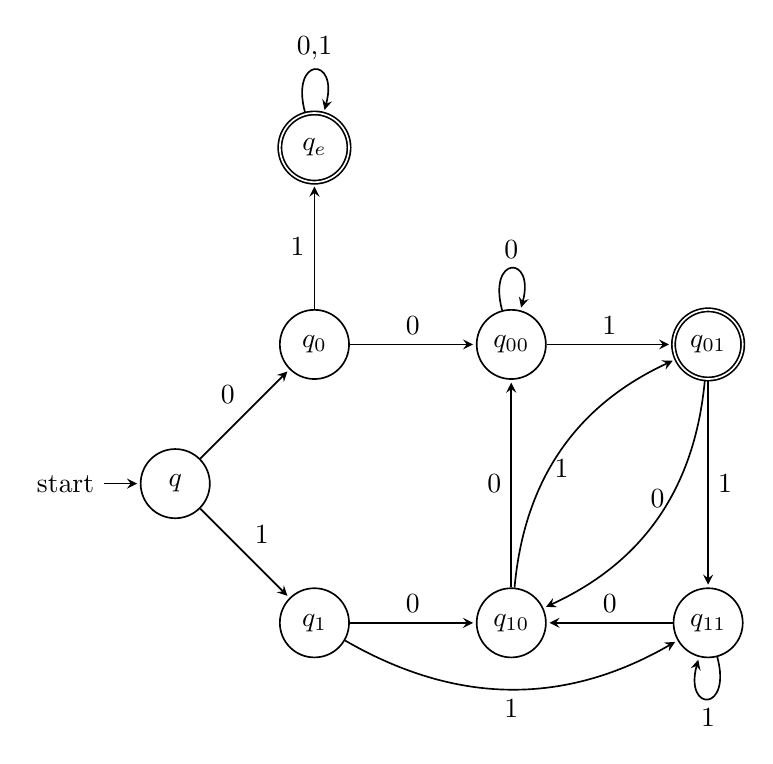
\begin{tikzpicture}[shorten >=1pt,->,>=stealth,semithick,node distance=2.5cm,auto]
\node[state,initial] (q) {$q$};
\node[state] (q_0) [above right of=q] {$q_0$};
\node[state,accepting] (q_e) [above of=q_0] {$q_e$};
\node[state] (q_1) [below right of=q] {$q_1$};
\node[state] (q_{00}) [right of=q_0] {$q_{00}$};
\node[state,accepting] (q_{01}) [right of=q_{00}] {$q_{01}$};
\node[state] (q_{10}) [right of=q_1] {$q_{10}$};
\node[state] (q_{11}) [right of=q_{10}] {$q_{11}$};

\path[->] (q) edge node {0} (q_0) edge node {1} (q_1)
(q_0) edge node {0} (q_{00}) edge node {1} (q_e)
(q_1) edge node {0} (q_{10}) edge [bend right] node [below] {1} (q_{11})
(q_e) edge [loop above] node {0,1} ()
(q_{00}) edge [loop above] node {0} () edge node {1} (q_{01})
(q_{01}) edge [bend left] node [above] {0} (q_{10}) edge node {1} (q_{11})
(q_{10}) edge node {0} (q_{00}) edge [bend left] node [below] {1} (q_{01})
(q_{11}) edge node [above] {0} (q_{10}) edge [loop below] node {1} ();
\end{tikzpicture}
\end{center}
\textbf{d)} I think empty string is also acceptable.\par
$A=(\{q_{i,j}:i\in\{0,1,2,3,4\},j\in\{0,1,2\}\},\{0,1\},\delta,q_{0,0},\{q_{0,0}\})$\par
$\delta(q_{i,j},0)=q_{(i+1)\mod 5,j},\delta(q_{i,j},1)=q_{i,(j+1)\mod 3}$
\end{exercise}

\begin{exercise}{2.2.6}\hspace{0pt}\\
\textbf{a)} 
\begin{center}
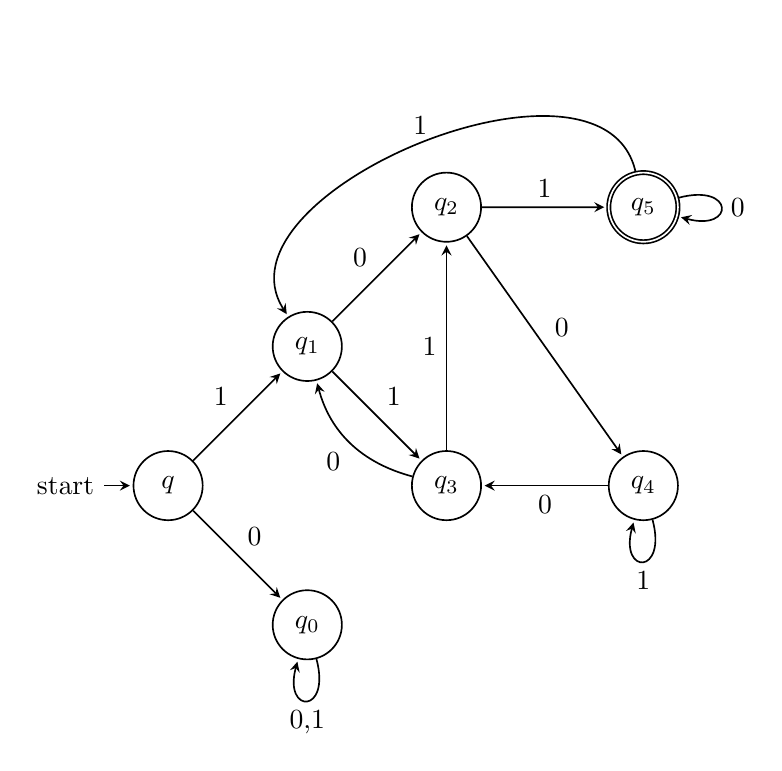
\begin{tikzpicture}[shorten >=1pt,->,>=stealth,semithick,node distance=2.5cm,auto,scale=0.8]
\node[state,initial] (q) {$q$};
\node[state] (q_0) [below right of=q] {$q_0$};
\node[state] (q_1) [above right of=q] {$q_1$};
\node[state] (q_2) [above right of=q_1] {$q_2$};
\node[state,accepting] (q_5) [right of=q_2] {$q_5$};
\node[state] (q_3) [below right of=q_1] {$q_3$};
\node[state] (q_4) [right of=q_3] {$q_4$};

\path[->] (q) edge node {0} (q_0) edge node {1} (q_1)
(q_0) edge [loop below] node {0,1} ()
(q_1) edge node {0} (q_2) edge node {1} (q_3)
(q_2) edge node {1} (q_5) edge node {0} (q_4)
(q_3) edge [bend left] node {0} (q_1) edge node {1} (q_2)
(q_4) edge node {0} (q_3) edge [loop below] node {1} ()
(q_5) edge [loop right] node {0} () edge [bend right=100] node [above] {1} (q_1);
\end{tikzpicture}
\end{center}
\textbf{b)} I think empty string is not acceptable.
\begin{center}
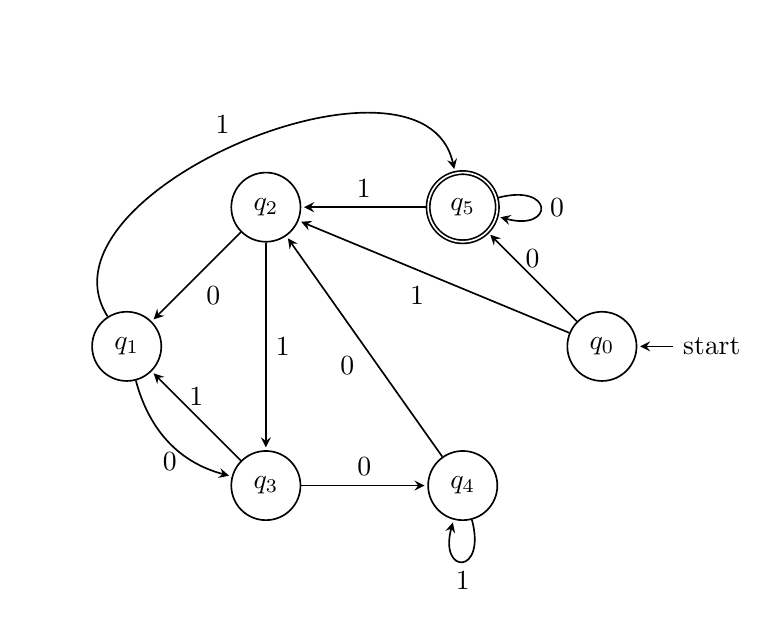
\begin{tikzpicture}[shorten >=1pt,->,>=stealth,semithick,node distance=2.5cm,auto]
\node[state] (q1) {$q_1$};
\node[state] (q2) [above right of=q1] {$q_2$};
\node[state,accepting] (q5) [right of=q2] {$q_5$};
\node[state] (q3) [below right of=q1] {$q_3$};
\node[state] (q4) [right of=q3] {$q_4$};
\node[state,initial right] (q0) [below right of=q5] {$q_0$};

\path[->] (q1) edge [bend right] node [below] {0} (q3) edge [bend left=100] node {1} (q5)
(q2) edge node {0} (q1) edge node {1} (q3)
(q3) edge node {0} (q4) edge node [above] {1} (q1)
(q4) edge node {0} (q2) edge [loop below] node {1} ()
(q5) edge [loop right] node {0} () edge node [above] {1} (q2)
(q0) edge node [above] {0} (q5) edge node {1} (q2);
\end{tikzpicture}
\end{center}
\end{exercise}

\begin{exercise}{2.2.9}\hspace{0pt}\\
\textbf{a)}
    Prove by induction.\par
    If $|w|=1$, $w=a\in\Sigma$. Then $\hat{\delta}(q_0,w)=\delta(q_0,a)=\delta(q_f,a)=\hat{\delta}(q_f,w)$.\par
    Assume $w=xa,|x|=k\geqslant 1$ and $\hat{\delta}(q_0,x)=\hat{\delta}(q_f,x)$. 
    By the definition of DFA, $\hat{\delta}(q_0,w)=\delta(\hat{\delta}(q_0,x),a)=\delta(\hat{\delta}(q_f,x),a)=\hat{\delta}(q_f,w)$.\\
\textbf{b)}
    Assume $x\neq\varepsilon\in L(A)$. Then by the definition of $L(A)$, $\hat{\delta}(q_0,x)=q_f$.
    Since $\hat{\delta}(q_0,w)=\hat{\delta}(q_f,w)$, $\hat{\delta}(q_0,x^k)=\hat{\delta}(\hat{\delta}(q_0,x),x^{k-1})=
    \hat{\delta}(q_f,x^{k-1})=\hat{\delta}(q_0,x^{k-1})$. By induction on $k$, $x^k\in L(A)$.
\end{exercise}

\begin{exercise}{2.2.10}
It accepts all $01$ string with odd number of $1$ in it.
\begin{proof}
    Assume $w$ is a nonempty $01$ string. Claim that \textit{$w$ with odd number of $1$ in it ends in state $B$,
    while $w$ with even number of $1$ in it ends in state $A$.} Prove by induction. \par
    If $|w|=1$, the claim is obviously correct.\par
    Assume $w=xa,|x|=k\geqslant 1,a\in\{0,1\}$. If $\hat{\delta}(x)=A$, there is even number of $1$ in $x$, then 
    $a=0$ will stick to $A$ and $a=1$ will change to $B$. Similar reasoning when $\hat{\delta}(x)=B$, which shows 
    the correctness of the claim in length of $k+1$.
\end{proof}
\end{exercise}

\begin{exercise}{2.2.11}
It accepts all $01$ string with no $00$ pattern in it.
\begin{proof}
    Assume $w$ is a $01$ string. If $w=\varepsilon$, it is obviously true. Let $w\neq\varepsilon$ in the following.
    Claim that \textit{
        $w$ with no $00$ in it and has $1$ as its last character ends in $A$.
        $w$ with no $00$ in it and has $0$ as its last character ends in $B$.
        $w$ with $00$ in it ends in $C$.
    } Prove by induction.\par
    If $|w|=1$, the claim is obviously correct.\par
    Assume $w=xa,|x|=k\geqslant 1,a\in\{0,1\}$. If $\hat{\delta}(x)=A$, there is no $00$ in $x$ and the last
    character of $x$ is $1$, then 
    $a=1$ will stick to $A$ and $a=0$ will change to $B$, which is correspondent with the claim.
    Similar reasoning when $\hat{\delta}(x)=B,C$, which shows 
    the correctness of the claim in length of $k+1$.
\end{proof}
\end{exercise}

\begin{exercise}{2.3.3}\hspace{0pt}\\
\begin{center}
\begin{tabular}{r || c | c}
& $0$ & $1$\\
\hline\hline
$\rightarrow p$ & $q$ & $p$\\
$q$ & $s$ & $r$\\
$*r$ & $q$ & $p$\\
$*s$ & $s$ & $r$
\end{tabular}
\end{center}
It accepts all the $01$ strings ending with $01$ or $00$.
\end{exercise}

\begin{exercise}{2.3.4}\hspace{0pt}\\
\textbf{a)} Denote $\Sset=\{0,1,2,\cdots,9\}$.
\begin{center}
\scalebox{0.9}{
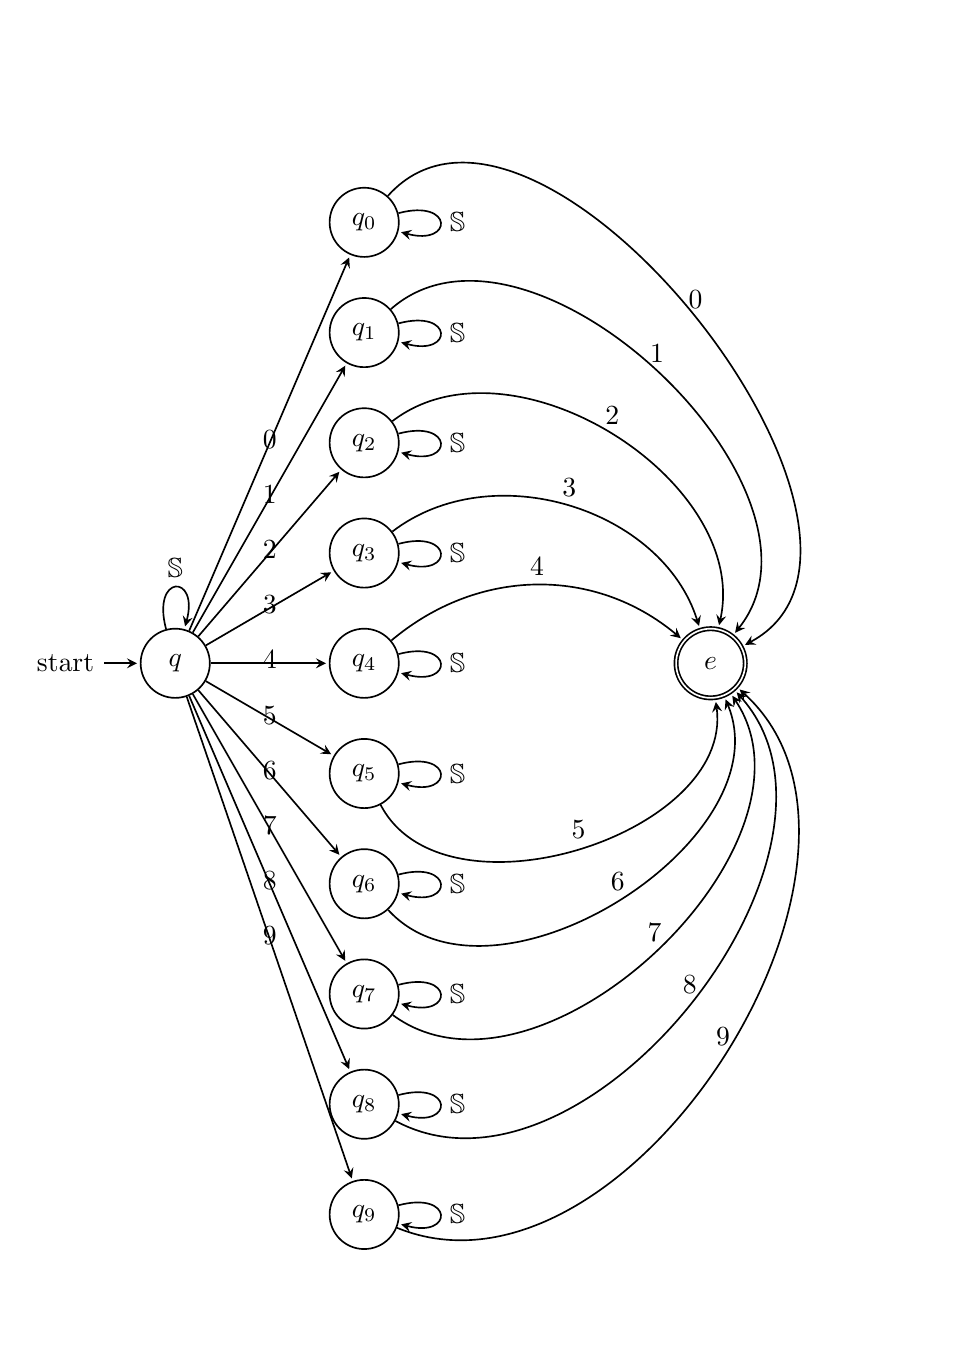
\begin{tikzpicture}[shorten >=1pt,->,>=stealth,semithick,node distance=1.4cm,auto]
    \node[state,initial] (q) {$q$};
    \path[->] (q) edge [loop above] node {$\Sset$} ();
    \node[state] (q4) [right of=q, xshift=1cm] {$q_4$};
    \node[state,accepting] (e) [right of=q4, xshift=3cm] {$e$};
    \foreach \x/\y in {3/4,2/3,1/2,0/1} 
        \node[state] (q\x) [above of=q\y] {$q_\x$};
    \foreach \x/\y in {5/4,6/5,7/6,8/7,9/8} 
        \node[state] (q\x) [below of=q\y] {$q_\x$};
    \foreach \x in {0,...,9}
        \path[->] (q) edge node [above,yshift=-2mm] {$\x$} (q\x);
    \foreach \x in {0,...,4}
        \path[->] (q\x) edge [bend left=100-\x*15] node [above] {$\x$} (e) edge [loop right] node {$\Sset$} ();
    \foreach \x in {5,...,9}
        \path[->] (q\x) edge [bend right=80] node [above] {$\x$} (e) edge [loop right] node {$\Sset$} ();
\end{tikzpicture}}
\end{center}
\textbf{b)} Denote $\Sset=\{0,1,2,\cdots,9\}$.
\begin{center}
\scalebox{0.9}{
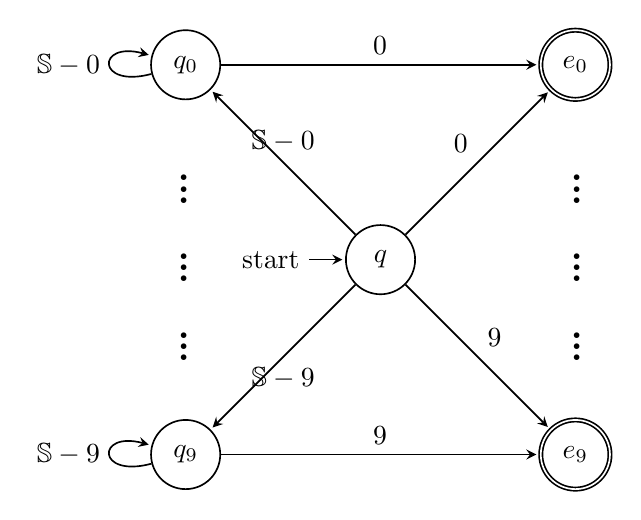
\begin{tikzpicture}[shorten >=1pt,->,>=stealth,semithick,node distance=3.5cm,auto]
    \node[state,initial] (q) {$q$};
    \node[state] (q0) [above left of=q] {$q_0$};
    \node[state,accepting] (e0) [above right of=q] {$e_0$};
    \node[state] (q9) [below left of=q] {$q_9$};
    \node[state,accepting] (e9) [below right of=q] {$e_9$};

    \path[->] (q) edge node [above] {$\Sset-0$} (q0) edge node [below] {$\Sset-9$} (q9) edge node {$0$} (e0) edge node {$9$} (e9)
    (q0) edge [loop left] node {$\Sset-0$} () edge node {$0$} (e0) 
    (q9) edge [loop left] node {$\Sset-9$} () edge node {$9$} (e9);

    \foreach \y in {-1cm,0cm,1cm} {
        \node [left of=q,xshift=1cm,yshift=\y] {\Huge\vdots};
        \node [right of=q,xshift=-1cm,yshift=\y] {\Huge\vdots};
    }
\end{tikzpicture}}
\end{center}
\textbf{c)}
\begin{center}
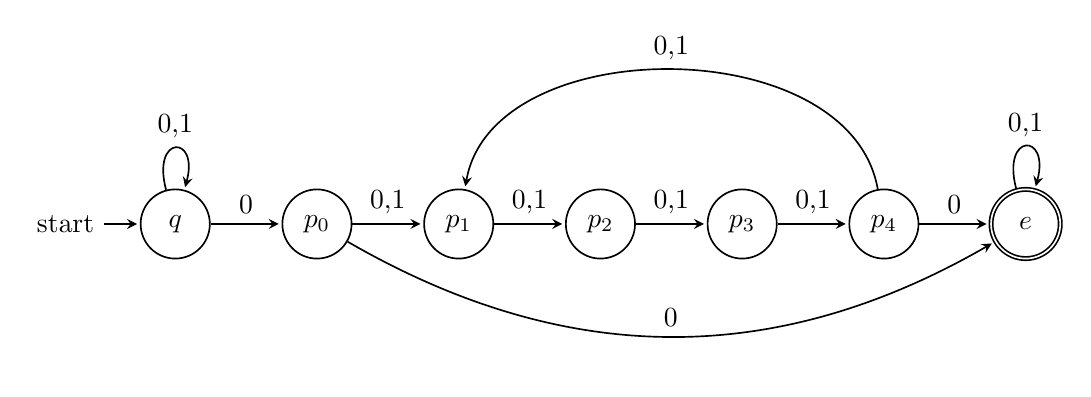
\begin{tikzpicture}[shorten >=1pt,->,>=stealth,semithick,node distance=1.8cm,auto]
    \node[state,initial] (q) {$q$};
    \node[state] (p0) [right of=q] {$p_0$};
    \node[state] (p1) [right of=p0] {$p_1$};
    \node[state] (p2) [right of=p1] {$p_2$};
    \node[state] (p3) [right of=p2] {$p_3$};
    \node[state] (p4) [right of=p3] {$p_4$};
    \node[state,accepting] (e) [right of=p4] {$e$};

    \path[->] (q) edge [loop above] node {0,1} (q) edge node {0} (p0)
    (p0) edge node {0,1} (p1) edge [bend right] node {0} (e)
    (p1) edge node {0,1} (p2)
    (p2) edge node {0,1} (p3)
    (p3) edge node {0,1} (p4)
    (p4) edge [bend right=80] node [above] {0,1} (p1) edge node {0} (e)
    (e) edge [loop above] node {0,1} ();
\end{tikzpicture}
\end{center}
\end{exercise}

\begin{exercise}{2.3.7}
    Assume $w$ is a nonempty string. Claim: \textit{$w$ ends in $q_i,i=1,2,\cdots,n$ if and only if the last $i$-th character of 
    $w$ is $1$}.
    \begin{proof}
        Prove by induction.\par
        If $|w|=1$, the claim is obviously correct.\par
        Assume $w=xa,|x|=k\geqslant 1,a\in\{0,1\}$ and $x$ ends in $q_j,j=0,1,\cdots,n$. 
        \begin{itemize}
            \item $j=0,a=1$, then next it can go to $q_0,q_1$. If it goes to $q_1$, the claim holds.
            \item $j=0,a=0$, then it goes to $q_0$.
            \item $0<j<n,a\in\{0,1\}$, then the last $j$-th character of $x$ is $1$. And afterwards $w$ goes to $q_{j+1}$ and the
                last $j+1$-th character of $w$ is $1$. The claim holds.
            \item $j=n,a\in\{0,1\}$, then it has no next way.
        \end{itemize}\par
        So the claim is true when the length is $k+1$.
    \end{proof}
\end{exercise}


\begin{exercise}{2.4.1}\hspace{0pt}\\
\textbf{a)} $q_2$ accepts abc; $q_6$ accepts abd; $q_5$ accepts aacd.
\begin{center}
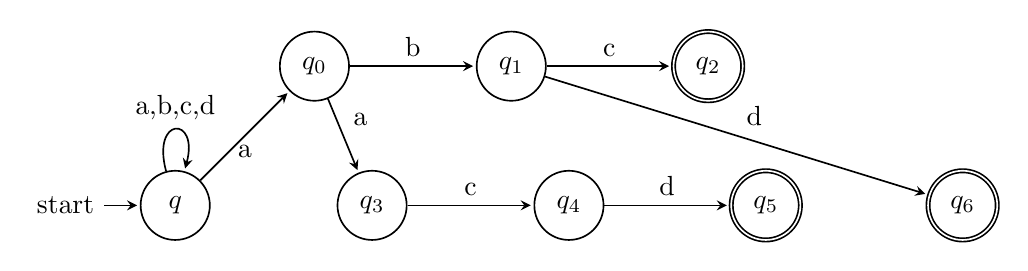
\begin{tikzpicture}[shorten >=1pt,->,>=stealth,semithick,node distance=2.5cm,auto]
\node[state,initial] (q) {$q$};
\node[state] (q0) [above right of=q] {$q_0$};
\node[state] (q1) [right of=q0] {$q_1$};
\node[state,accepting] (q2) [right of=q1] {$q_2$};
\node[state] (q3) [right of=q] {$q_3$};
\node[state] (q4) [right of=q3] {$q_4$};
\node[state,accepting] (q5) [right of=q4] {$q_5$};
\node[state,accepting] (q6) [right of=q5] {$q_6$};

\path[->] (q) edge [loop above] node {a,b,c,d} () edge node [below] {a} (q0)
(q0) edge node {b} (q1) edge node {a} (q3)
(q1) edge node {c} (q2) edge node {d} (q6) 
(q3) edge node {c} (q4)
(q4) edge node {d} (q5);
\end{tikzpicture}
\end{center}
\textbf{b)} $q_4$ accepts 011; $q_3$ accepts 0101; $q_7$ accepts 101.
\begin{center}
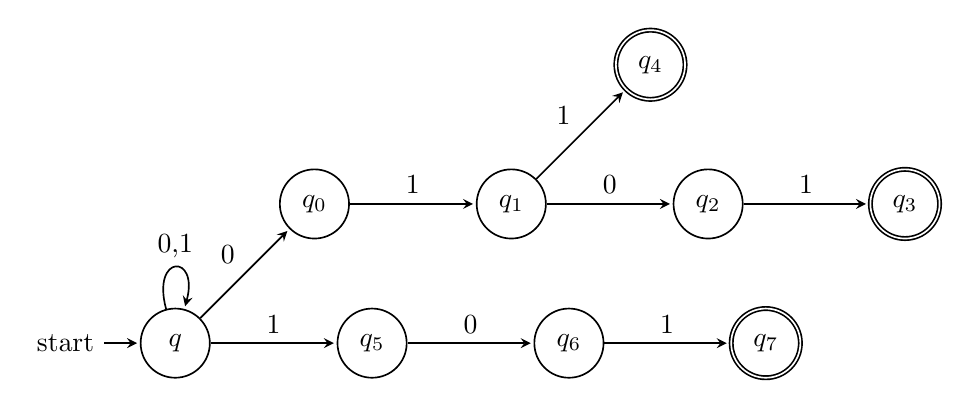
\begin{tikzpicture}[shorten >=1pt,->,>=stealth,semithick,node distance=2.5cm,auto]
\node[state,initial] (q) {$q$};
\node[state] (q0) [above right of=q] {$q_0$};
\node[state] (q1) [right of=q0] {$q_1$};
\node[state] (q2) [right of=q1] {$q_2$};
\node[state,accepting] (q3) [right of=q2] {$q_3$};
\node[state,accepting] (q4) [above right of=q1] {$q_4$};
\node[state] (q5) [right of=q] {$q_5$};
\node[state] (q6) [right of=q5] {$q_6$};
\node[state,accepting] (q7) [right of=q6] {$q_7$};

\path[->] (q) edge [loop above] node {0,1} () edge node {0} (q0) edge node {1} (q5)
(q0) edge node {1} (q1) 
(q1) edge node {0} (q2) edge node {1} (q4) 
(q2) edge node {1} (q3) 
(q5) edge node {0} (q6)
(q6) edge node {1} (q7);
\end{tikzpicture}
\end{center}
\textbf{c)} $q_1$ accepts ab; $q_3$ accepts bc; $q_5$ accepts ca.
\begin{center}
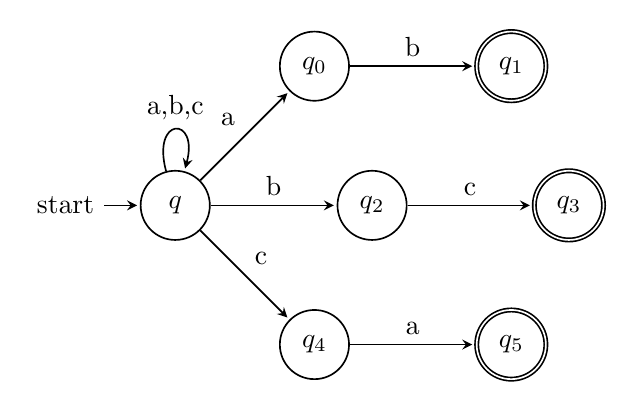
\begin{tikzpicture}[shorten >=1pt,->,>=stealth,semithick,node distance=2.5cm,auto]
\node[state,initial] (q) {$q$};
\node[state] (q0) [above right of=q] {$q_0$};
\node[state,accepting] (q1) [right of=q0] {$q_1$};
\node[state] (q2) [right of=q] {$q_2$};
\node[state,accepting] (q3) [right of=q2] {$q_3$};
\node[state] (q4) [below right of=q] {$q_4$};
\node[state,accepting] (q5) [right of=q4] {$q_5$};

\path[->] (q) edge [loop above] node {a,b,c} () edge node {a} (q0) edge node {b} (q2) edge node {c} (q4)
(q0) edge node {b} (q1)
(q2) edge node {c} (q3)
(q4) edge node {a} (q5);
\end{tikzpicture}
\end{center}
\end{exercise}

\begin{exercise}{2.4.2}\hspace{0pt}\\
\textbf{a)} $q_2$ accepts abc; $q_3$ accepts abd; $q_6$ accepts aacd.
\begin{center}
\begin{tabular}{r || c | c | c | c}
& $a$ & $b$ & $c$ & $d$\\
\hline\hline
    $\rightarrow q$ & $q_0$ & $q$ & $q$ & $q$\\
    $q_0$ & $q_4$ & $q_1$ & $q$ & $q$\\
    $q_1$ & $q_0$ & $q$ & $q_2$ & $q_3$\\
    $*q_2$ & $q_0$ & $q$ & $q$ & $q$\\
    $*q_3$ & $q_0$ & $q$ & $q$ & $q$\\
    $q_4$ & $q_4$ & $q_1$ & $q_5$ & $q$\\
    $q_5$ & $q_0$ & $q$ & $q$ & $q_6$\\
    $*q_6$ & $q_0$ & $q$ & $q$ & $q$\\
\end{tabular}
\end{center}
\textbf{b)} $q_3$ accepts 0101 and 101; $q_4$ accepts 011; $q_7$ accepts 101.
\begin{center}
\begin{tabular}{r || c | c }
& $0$ & $1$\\
\hline\hline
    $\rightarrow q$ & $q_0$ & $q_5$\\
    $q_0$ & $q_0$ & $q_1$ \\
    $q_1$ & $q_2$ & $q_4$ \\
    $q_2$ & $q_0$ & $q_3$ \\
    $*q_3$ & $q_2$ & $q_4$ \\
    $*q_4$ & $q_6$ & $q_5$ \\
    $q_5$ & $q_6$ & $q_5$ \\
    $q_6$ & $q_0$ & $q_7$ \\
    $*q_7$ & $q_2$ & $q_4$ \\
\end{tabular}
\end{center}
\textbf{c)} $q_1$ accepts ab; $q_3$ accepts bc; $q_5$ accepts ca.
\begin{center}
\begin{tabular}{r || c | c | c }
& $a$ & $b$ & $c$\\
\hline\hline
    $\rightarrow q$ & $q_0$ & $q_2$ & $q_4$\\
    $q_0$ & $q_0$ & $q_1$ & $q_4$\\
    $*q_1$ & $q_0$ & $q_2$ & $q_3$ \\
    $q_2$ & $q_0$ & $q_2$ & $q_3$\\
    $*q_3$ & $q_5$ & $q_2$ & $q_4$ \\
    $q_4$ & $q_5$ & $q_2$ & $q_4$\\
    $*q_5$ & $q_0$ & $q_1$ & $q_4$ \\
\end{tabular}
\end{center}
\end{exercise}

\begin{exercise}{2.5.1}\hspace{0pt}\\
\textbf{a)}
\begin{center}
\begin{tabular}{c || c}
STATE & ECLOSE\\
\hline\hline
$p$ & $\{p\}$\\
$q$ & $\{q,p\}$\\
$r$ & $\{r,q,p\}$\\
\end{tabular}
\end{center}
\textbf{b)} c,ac,bb,bc,ca,cb,cc,aac,abb,abc,aca,acb,acc,bab,bac,bba,bbb,bbc,bca,bcb,bcc,caa,cab,cac,cba,cbb,cbc,cca,ccb,ccc\\
\textbf{c)}
\begin{center}
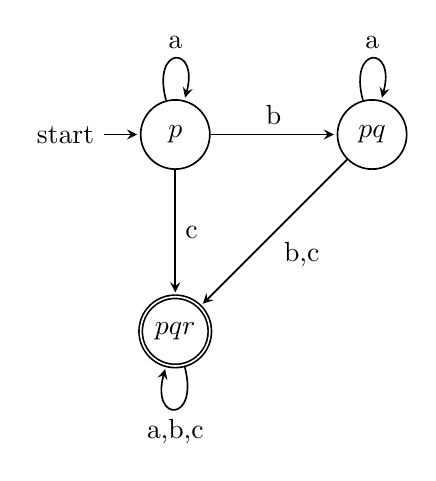
\begin{tikzpicture}[shorten >=1pt,->,>=stealth,semithick,node distance=2.5cm,auto]
\node[state,initial] (p) {$p$};
\node[state] (pq) [right of=p] {$pq$};
\node[state,accepting] (pqr) [below of=p] {$pqr$};

\path[->] (p) edge [loop above] node {a} () edge node {b} (pq) edge node {c} (pqr)
(pq) edge [loop above] node {a} () edge node {b,c} (pqr)
(pqr) edge [loop below] node {a,b,c} ();
\end{tikzpicture}
\end{center}
\end{exercise}

\begin{exercise}{2.5.3}\hspace{0pt}\\
\textbf{a)} I think empty string is acceptable.
\begin{center}
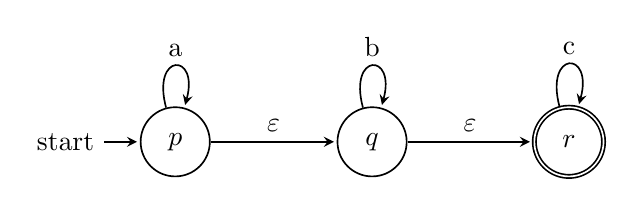
\begin{tikzpicture}[shorten >=1pt,->,>=stealth,semithick,node distance=2.5cm,auto]
\node[state,initial] (p) {$p$};
\node[state] (q) [right of=p] {$q$};
\node[state,accepting] (r) [right of=q] {$r$};

\path[->] (p) edge [loop above] node {a} () edge node {$\varepsilon$} (q)
(q) edge [loop above] node {b} () edge node {$\varepsilon$} (r)
(r) edge [loop above] node {c} ();
\end{tikzpicture}
\end{center}
\textbf{b)}
\begin{center}
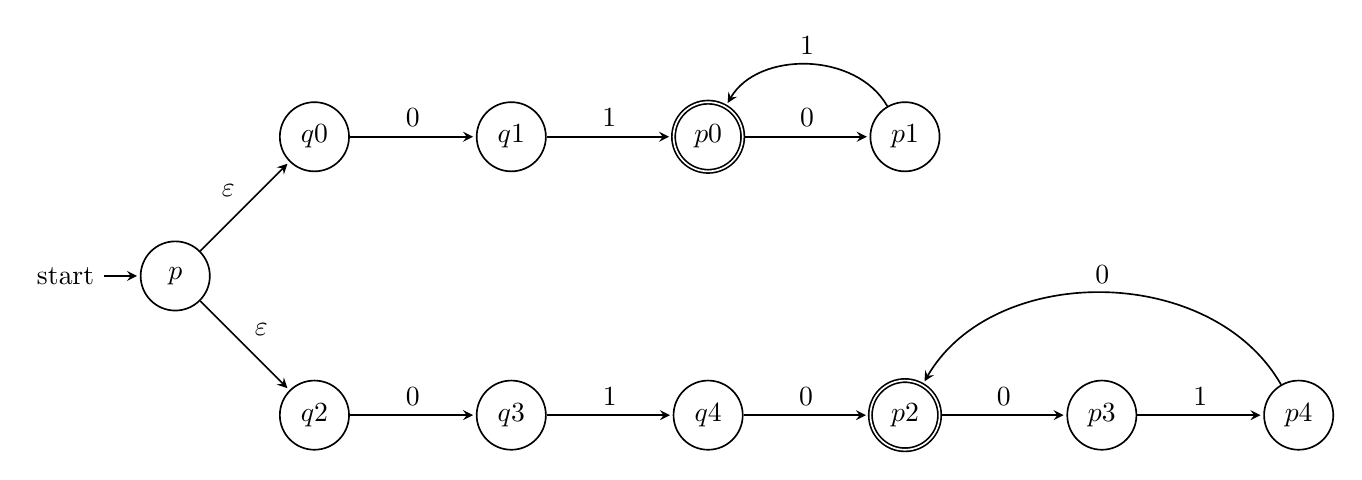
\begin{tikzpicture}[shorten >=1pt,->,>=stealth,semithick,node distance=2.5cm,auto]
\node[state,initial] (p) {$p$};
\node[state] (q0) [above right of=p] {$q0$};
\node[state] (q1) [right of=q0] {$q1$};
\node[state,accepting] (p0) [right of=q1] {$p0$};
\node[state] (p1) [right of=p0] {$p1$};
\node[state] (q2) [below right of=p] {$q2$};
\node[state] (q3) [right of=q2] {$q3$};
\node[state] (q4) [right of=q3] {$q4$};
\node[state,accepting] (p2) [right of=q4] {$p2$};
\node[state] (p3) [right of=p2] {$p3$};
\node[state] (p4) [right of=p3] {$p4$};

\path[->] (p) edge node {$\varepsilon$} (q0) edge node {$\varepsilon$} (q2)
(q0) edge node {0} (q1)
(q1) edge node {1} (p0)
(p0) edge node {0} (p1)
(p1) edge [bend right=60] node [above] {1} (p0)
(q2) edge node {0} (q3)
(q3) edge node {1} (q4)
(q4) edge node {0} (p2)
(p2) edge node {0} (p3)
(p3) edge node {1} (p4)
(p4) edge [bend right=60] node [above] {0} (p2);
\end{tikzpicture}
\end{center}
\textbf{c)} I think string of length less than $10$ is not acceptable.
\begin{center}
\scalebox{0.8}{
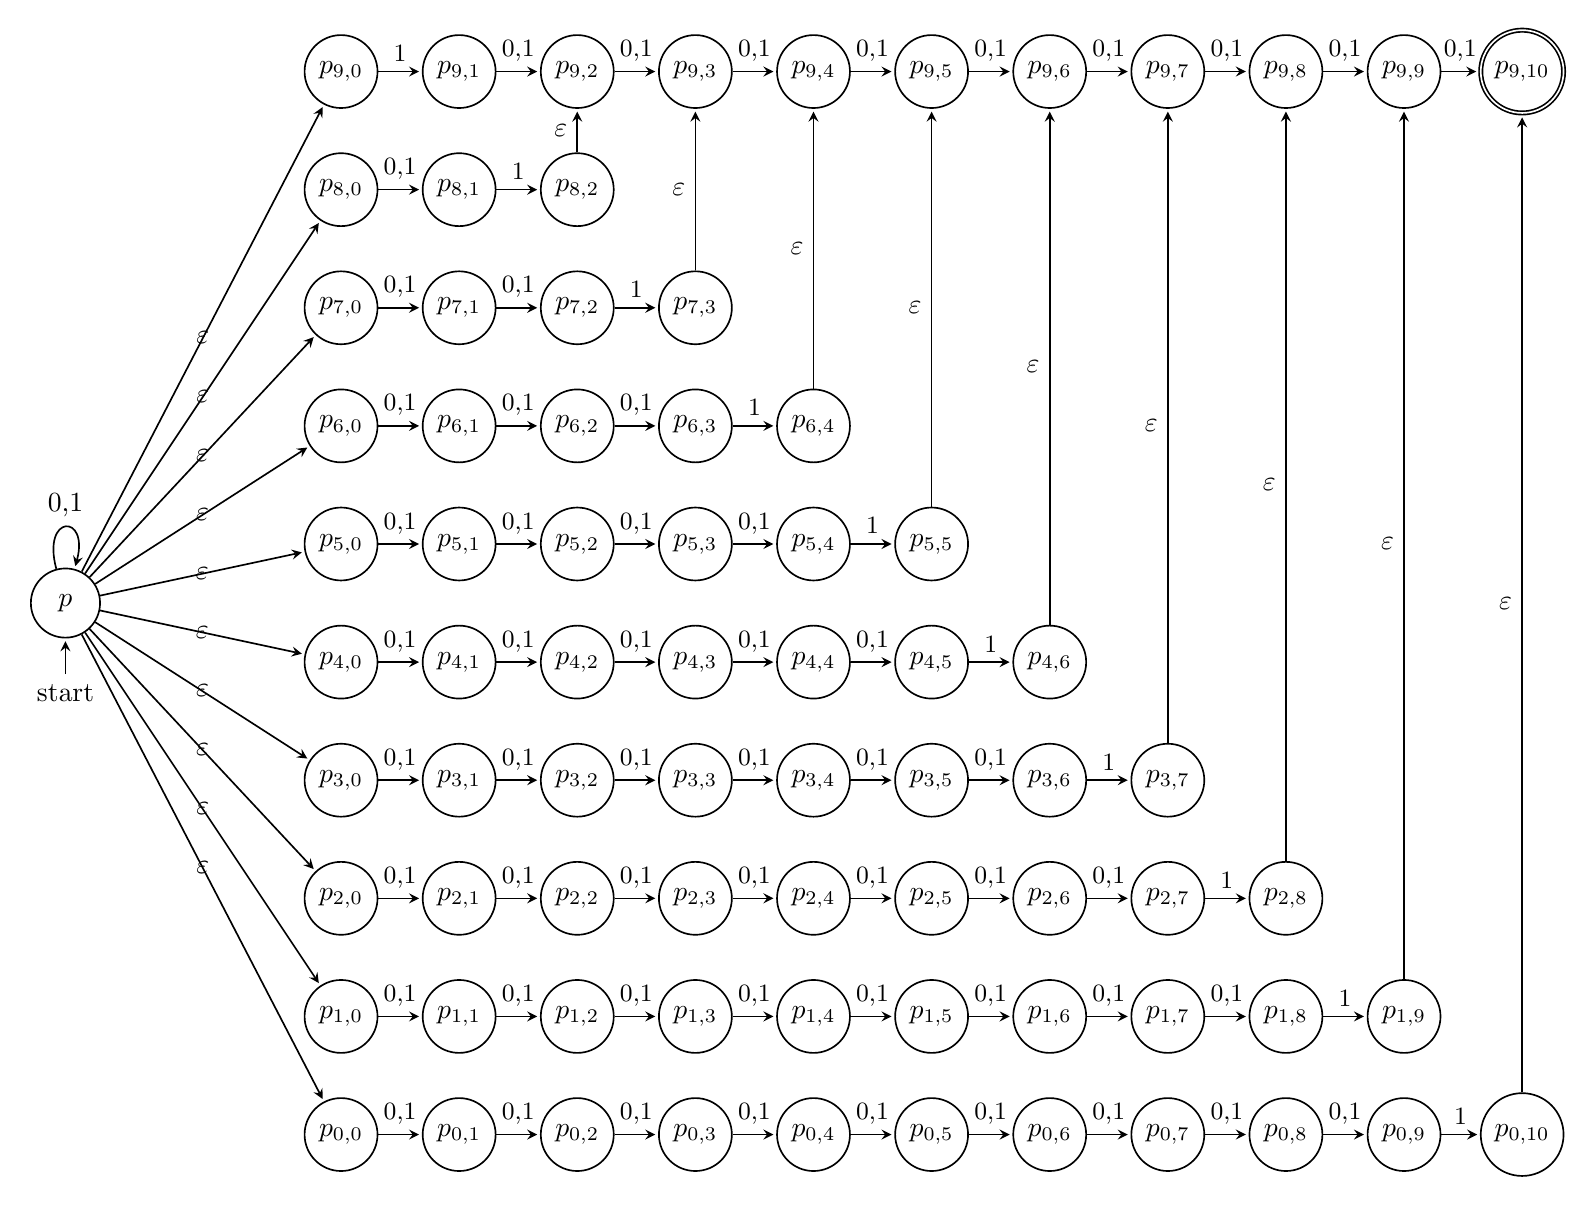
\begin{tikzpicture}[shorten >=1pt,->,>=stealth,semithick,node distance=1.5cm,auto]
\node[state,initial below] (p) at (-3.5,4.5*1.5) {$p$};
\path[->] (p) edge [loop above] node {0,1} ();
\foreach \x [evaluate=\x as \y using \x*1.5,remember=\x as \pre] in {0,...,10}{
    \ifnum \x=10
        \node[state,accepting] (p-9-\x) at (\y,9*1.5) {$p_{9,\x}$};
    \else
        \node[state] (p-9-\x) at (\y,9*1.5) {$p_{9,\x}$};
    \fi

    \ifnum \x>1
        \path[->] (p-9-\pre) edge node {\small 0,1} (p-9-\x);
    \else
        \ifnum \x=1
            \path[->] (p-9-\pre) edge node {\small 1} (p-9-\x);
        \fi
    \fi
}
\foreach \y [evaluate=\y as \z using 9-\y] in {0,...,8}
    \foreach \x [remember=\x as \pre] in {0,...,10}{
        \node[state] (p-\y-\x) at (\x*1.5,\y*1.5) {$p_{\y,\x}$};

        \ifnum \x>0
            \ifnum \x>\z
                \path[->] (p-\y-\pre) edge node {\small 1} (p-\y-\x);
            \else
                \path[->] (p-\y-\pre) edge node {\small 0,1} (p-\y-\x);
            \fi
        \fi
        
        \ifnum \x>\z
            \path[->] (p-\y-\x) edge node {$\varepsilon$} (p-9-\x);
            \breakforeach
        \fi
    }
\foreach \x in {0,...,9}
    \path[->] (p) edge node [above,yshift=-2mm] {$\varepsilon$} (p-\x-0);
    
\end{tikzpicture}}
\end{center}
\end{exercise}


\end{document}
